\chapter{Discussion} \label{cpt-discussion}

The following chapter discusses possible advantages and disadvantages of the proposed approach based on 
the data presented in Chapter \ref{cpt-experiment}. The results are revisited and summarized before they 
are interpreted and evaluated. Finally, limitations of the approach are presented and discussed.

\section{Summary of the Results}

The experiment tested the ability of the \ac{TPOC} to be adapted to a new use case. The traditional way of 
using \ac{TPOC} relies on preprocessing large objects that are usually artist-picked and are generally used 
in applications that make use of triangle meshes with only a boundary representation. This way, a lot of 
small objects can be occluded by one large occluder. In contrast, the algorithm cannot be applied to voxel 
rendering as is, since in a voxel scene there are only uniform meshes. Individual models might be interpreted 
as large occluders but they are generally very computational intense to draw because of their voxelized nature. \\

\noindent
In consequence, the \ac{TPOC} was adjusted to fit the spicific circumstances found in volumetric voxel representations. 
The uniform size of voxels made the traditional \ac{TPOC} rather inefficient in practice but the problem was 
successfully tackled by aggregating neighboring voxels to larger primitives, consequently decreasing computation 
time of the depth prepass. This approach also shifted the use of the algorithm slightly. Traditionally, \ac{TPOC} 
draws a handful of the best occluders to enable culling of emph{other} meshes. In the approach proposed in this work, 
the best occluders are part of the occluded model, and the geometry contributing to their creation may 
\emph{itself} be occluded. \\

\noindent
Overall, the experiment showed that the \ac{TPOC} algorithm can be customized to work in a volumetric voxel 
representation using two different configurations: the per-octree node culling and the per-meshlet culling. 
Both configurations were able to occlude a considerable amount of voxels while using a minimal amount of 
\ac{GPU} bandwidth. The per-meshlet culling was able to cull more octree nodes and, consequently, more 
voxels than the per-octree node culling. \\

\noindent
Using uniform voxels as primitives for approximating scene data, enables the complete creation of geometry on the 
\ac{GPU}. This also fits perfectly into the use of the mesh shading pipeline, since meshlets created on-chip do 
not have to be pre-computed. The creation of a large amount of geometry is therefore efficient and easy to 
implement. \\

\noindent
The \ac{CPU} times were found to be rather static, although both testing setups were not significantly reliant 
on \ac{CPU} computations due to their \ac{GPU}-driven nature. However, the \ac{GPU} measurements were significantly 
in favor of the \ac{PMOC} configuration, which overall increased performance by $29.86\%$ on 
average. \\

\noindent
The overdraw measurements showed varying overdraw values for both configurations, which resulted in a similar amount 
of overdraw in the best case. In the worst case, the per-meshlet culling generally resulted in lower overdraw than 
the per-octree node culling. The amount of overdraw reached up to a maximum of about 90 draws to one pixel for 
per-octree culling and up to about 70 draws to one pixel for per-meshlet culling. It strongly correlated to the 
camera angle and was considerably high in both configurations. \\ 

\noindent
The type of mesh used in the scene had a significant influence on both the culling efficiency and the computation time.
Large, dense models were generally favored and resulted in a high best occluder count. In contrast, curved edges or 
surfaces resulted in a low octree node occupation, which in turn led to high overdraw. Thin and detailed geometry or 
models featuring a lot of holes and empty space in them were rather inefficient in computation. They generally resulted 
in a lack of full octree nodes and therefore in a lower best occluder count and octree node occupation. Such models 
were found to be very sensitive to different camera angles and could not cull voxels as efficiently compared to the 
other models tested. Still, they would benefit from the culling algorithm in both configurations.

\section{Interpretation of the Results}

This work aimed to test if the \ac{TPOC} algorithm could be applied to voxel rendering by adopting a good approximation 
for the creation of the best occluders and if the use of the mesh shading pipeline would optimize the performance and 
the amount of culled voxels. The presented results indicate that this was successful. Nevertheless, the results also 
provide more in-depth insights that are discussed below. \\

\noindent
First of all, the results need to be considered in the correct context. This approach was tested with a particular use case 
in mind. The main constraint is the volumetric nature of the scene, which is essential for this algorithm to make sense in 
the first place. For non-volumetric representations, other occlusion culling algorithms might be better suited, or the 
selection of the best occluders would fall back to whole models instead of parts of a volumetric model, like in this work's 
implementation. Another constraint is the rasterized rendering pipeline, since the occlusion algorithm cannot be applied to 
raytraced rendering. If both of these essential requirements are satisfied, the proposed approach can be adopted, and the 
presented results can be used as a benchmark in terms of performance and culling results. \\

\noindent
The main factors to influence the resulting performance and the culling efficiency are the models and their voxel resolution.
In general, large bodies with large volumes can be approximated better than small or thin bodies. Models featuring small and 
thin details, holes, or large areas without geometry are harder to approximate. The higher the number of best occluders, the 
more likely it is that a lot of voxels are going to be culled in any given moment. \\

\noindent
But there are more nuanced relationships between the scene data and the performance. The \ac{GPU} performance scaled considerably 
with the amount of occluded voxels and, consequently, with the amount of visible voxels. The depth prepass scaled with the amount 
of best occluders that were drawn to the depth buffer, while the \ac{HiZ} creation wasn't shown to be scaling in the experiment, 
using a fixed screen resolution. Since in general, the \ac{HiZ} is the same for any given scene with the same screen resolution, 
it should only be impacted by a change of the screen resolution. This assumption is strongly supported by the way the \ac{HiZ} 
creation is implemented. Consequently, the final performance of both tested configurations is expected to vary based on the amount 
of completely filled octree nodes. \\

The data indicates that a higher average occupation has the tendency to result in better overall culling performance and subsequently 
in better \ac{GPU} performance as well. It can also be derived that the average culling efficiency increases with the increase of 
voxels in the scene. But this is only true to an extent, since the \emph{Hairball} model showed a decrease in average culling efficiency 
compared to the \emph{Lucy} model while having almost 5 times the voxel count. This tendency is therefore only visible for models 
that are similarly dense in structure and do not contain holes or other challenging features.\\

\begin{figure}[!htb]
    \centering
    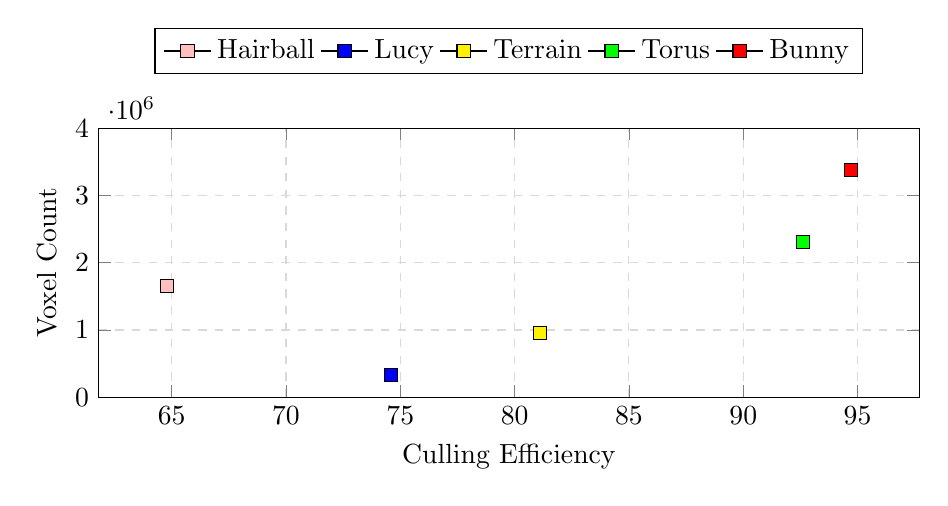
\begin{tikzpicture}
        \begin{axis}[
            width=12cm,
            height=5cm,
            ylabel={Voxel Count},
            xlabel={Culling Efficiency},
            grid=major,
            grid style={dashed, gray!30},
            legend style={at={(0.5,1.2)}, anchor=south, legend columns=5},
            ymin=0, ymax=4000000,
            scaled x ticks=false,
            ]
        
            \addplot[mark=square*, mark options={scale=1.2, fill=pink},] coordinates  {(64.8, 1652435)};
            \addplot[mark=square*, mark options={scale=1.2, fill=blue},] coordinates {(74.6, 331254)};
            \addplot[mark=square*, mark options={scale=1.2, fill=yellow},] coordinates {(81.1, 953362)};
            \addplot[mark=square*, mark options={scale=1.2, fill=green},] coordinates {(92.6, 2311006)};
            \addplot[mark=square*, mark options={scale=1.2, fill=red},] coordinates {(94.7, 3379738)};
            \legend{Hairball, Lucy, Terrain, Torus, Bunny}
        \end{axis}
    \end{tikzpicture}

    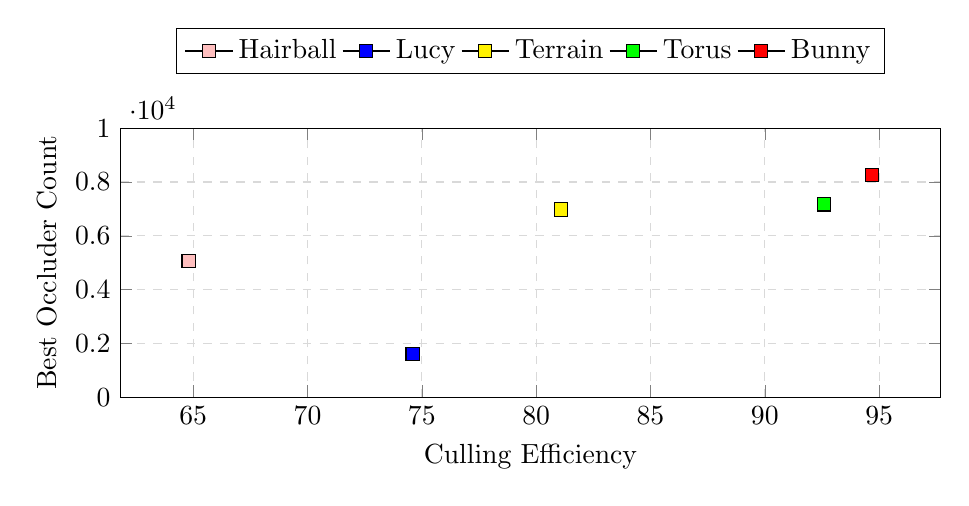
\begin{tikzpicture}
        \begin{axis}[
            width=12cm,
            height=5cm,
            ylabel={Best Occluder Count},
            xlabel={Culling Efficiency},
            grid=major,
            grid style={dashed, gray!30},
            legend style={at={(0.5,1.2)}, anchor=south, legend columns=5},
            ymin=0, ymax=10000,
            scaled x ticks=false,
            ]

            \addplot[mark=square*, mark options={scale=1.2, fill=pink},] coordinates  {(64.8, 5056)};
            \addplot[mark=square*, mark options={scale=1.2, fill=blue},] coordinates {(74.6, 1600)};
            \addplot[mark=square*, mark options={scale=1.2, fill=yellow},] coordinates {(81.1, 6976)};
            \addplot[mark=square*, mark options={scale=1.2, fill=green},] coordinates {(92.6, 7168)};
            \addplot[mark=square*, mark options={scale=1.2, fill=red},] coordinates {(94.7, 8256)};
            \legend{Hairball, Lucy, Terrain, Torus, Bunny}
        \end{axis}
    \end{tikzpicture}
    \caption{Upper: The relation between voxel count and culling efficiency.
    Lower: The relation between best occluder count and culling efficiency.}
    \label{plt:culling-efficiency-voxel-node-count}
\end{figure}

\noindent
The general approximation of best occluders did work well for most of the models. However, the \emph{Hairball} model showed that specific 
features posed a challenge for the algorithm. The approximation of a model's volume by aggregating voxels together is only possible for 
models that provide dense volumes in the first place. The systematic testing of a challenging model provided valuable insights into the 
limitations of the approach. Consequently, the algorithm is expected to not be very beneficial when using it in scenes with small, thin 
details or holes.\\




%\noindent [@TODO: Consider moving this to technical background or something like this]
%The fact that the approach uses screen space visibility testing results in a general purpose culling algorithm. Although there are use cases 
%in which the approach works better than in others, there is limitation to where it can be applied. Consider another occlusion culling algorithm 
%that uses bouding boxes to approximate object boundaries. Such an algorithm would check for visibility using the bounding volumes. If one of the 
%objects were a wall with a window in it, this could not be reliably computed because of the hole in the wall. Another technique would have to 
%be used here in order to test for visibility using the \\

\noindent
The \ac{TPOC} algorithm usually uses a handful of occluders to cull other occludees. So normally, there is no overlap between occluders and 
occludees. However, this work's approach uses a slightly different way of working with occluders and occludees. Because of their volumetric 
nature, the models can self-occlude, which means that the approximated volume can be used as an occluder to cull a vast amount of voxels that 
make up the volume itself. This is a slightly different perspective on the \ac{TPOC} algorithm and makes it possible to use the approach when 
there is only one model present. \\

\noindent
The per-meshlet culling configuration proved to be more efficient due to a more precise culling of voxels, even partially culling octree nodes.
In this sense, the mesh shading pipeline featured a higher culling ratio and superior occlusion culling in general. Another aspect to consider 
is the possibility of optimizing the \ac{HZB} algorithm further. Traditionally, when comparing a bounding box to the \ac{HiZ} pyramid, all depth 
values of the \ac{HiZ} pyramid within the minimum and maximum bounds need to be checked against the minimum z value of the object in question.
This is where the hierarchy optimizes the process because with each mip level, a texel covers a greater section of the depth buffer, making 
sampling the \ac{HiZ} pyramid cheaper in terms of computation time. Since cubical voxels are easily defined by their min and max values and 
there is no sub-voxel detail, this process can potentially be optimized further. When using per-meshlet culling, each voxel's bounds are 
checked individually, and theoretically, no hierarchy is necessary. This assumption was formed by this work's implementation, since it only used 
the full-resolution depth buffer for the \ac{HZB} due to visual errors that couldn't be fixed in time. That way, only one sampling per screen 
rectangle corner is necessary, either per mip level, or only using the full resolution z-buffer. If this assumption holds true and can be 
generally confirmed, the computation of the prepass would reduce to only the depth pass, without the need to compute a hierarchy. \\

\noindent
No matter how the prepass is executed, the measurements show that the highly parallelized way of computing the occlusion test does not lead to 
the per-meshlet culling being slower than the per-octree culling. This can be explained by the massive amount of parallelization that is 
possible in modern hardware and how the more fine-grained culling removes more geometry than the per-octree node culling does. This in turn leads 
to a lower dispatch count of mesh shaders and subsequently to a lower load on rasterizer and pixel shader computations. However, this relation 
is expected to be only valid for a reasonable amount of dispatches by the task shader, since a higher amount could ultimately lead to an inefficient 
usage of \ac{GPU} threads. \\

\noindent
The \ac{GPU}-driven approach moves most of the computations for the occlusion culling to the \ac{GPU}, leaving more \ac{CPU} cycles for different 
computations, like updating the voxel data dynamically. When using the approach with suitable scenes and geometry, this algorithm might be able 
to optimize volumetric voxel rendering further. Particularly if the proposed implementation is even further optimized to fit the given use case, 
for example, by using command lists to avoid a write-back to \ac{CPU} memory before dispatching the meshes for the final draw call. \\



\section{Limitations}

The experiment also featured some limitations that are essential to consider for further research of the approach.
A central limitation was the depth hierarchy, which was not being used in the intended way, as mentioned earlier.
Due to unresolvable visual errors, the full-resolution depth buffer was used for the visibility checks, however, 
using the full depth pyramid should usually yield similar or better results in terms of runtime performance. 
Nevertheless, this limited the precision of the measurements in a way that the depth prepass couldn't be measured 
in its full complexity. As the data suggests, the major differences in the compared pipeline configurations were 
originating from the \emph{DispatchMesh} routine, which was not influenced by the actual implementation of the 
depth prepass. \\

\noindent
Another limitation was introduced by the hardware limitations in the mesh shading pipeline, or, more specifically, the 
compute shader architecture. Due to the maximum amount of threadgroups that could be scheduled on the \ac{GPU}, there 
was a limit to how many octree nodes could be computed within one draw call. Since the amount of voxels was equal to the 
amount of threads scheduled in the shader, the model resolution was limited by the experimental setup, which only used 
one draw call for better comparability. This limitation also meant, that the \ac{GPU} utilization varied quite a lot. 
In the given implementation, rejecting a large amount of octree nodes or voxels would consequently mean that the 
threadgroups and threads would exit early. A more in-depth evaluation of this behaviour is necessary to find out if 
there is a more efficient way to computing the voxels using the mesh shading piepeline. \\

\noindent
As mentioned before, a major limitation is the overdraw within the pipeline. Although it could be shown that the 
computation time can be reduced compared to the \ac{PONOC}, the maximum overdraw is still 
very high. This is due to the best occluders which are not able to cull all occluded voxels but will rather cull 
most of the occluded voxels. It is up to further inspection if the amount of overdraw is bearable for a given use 
case, or if it is too much overdraw. \\

\noindent
Although it is possible to handle multiple models without any changes to the pipeline, the limitation of a maximum 
dispatch count mentioned before needs to be considered here. When having multiple seperate models within the scene, 
how good the culling works really depends on the models, their properties, and the scene's resolution. In general, 
any best occluder can cull voxels of any given model. But the more best occluders present in the scene, the more 
the depth prepass will scale to longer computation times. For better performance, it might serve well to chunk the 
scene and only consider the best occluders within "active" chunks for the culling. Chunking the scene is also 
expected to be of advantage for dynamically updating the voxel data and therefore the best occluder data. For this 
particular work, the management of chunk data is handled by the \ac{CPU}, which means that updating the data could 
potentially be parallelized on the \ac{CPU} by using scene chunks. \\
 